\documentclass[border=10pt]{standalone}

\usepackage{tikz}
\usepackage{tikzsymbols}
\usetikzlibrary{calc,patterns,shapes.geometric}

\def\centerarc[#1](#2)(#3:#4:#5){\draw[#1] ($(#2)+({#5*cos(#3)},{#5*sin(#3)})$) arc (#3:#4:#5);}

\begin{document}
	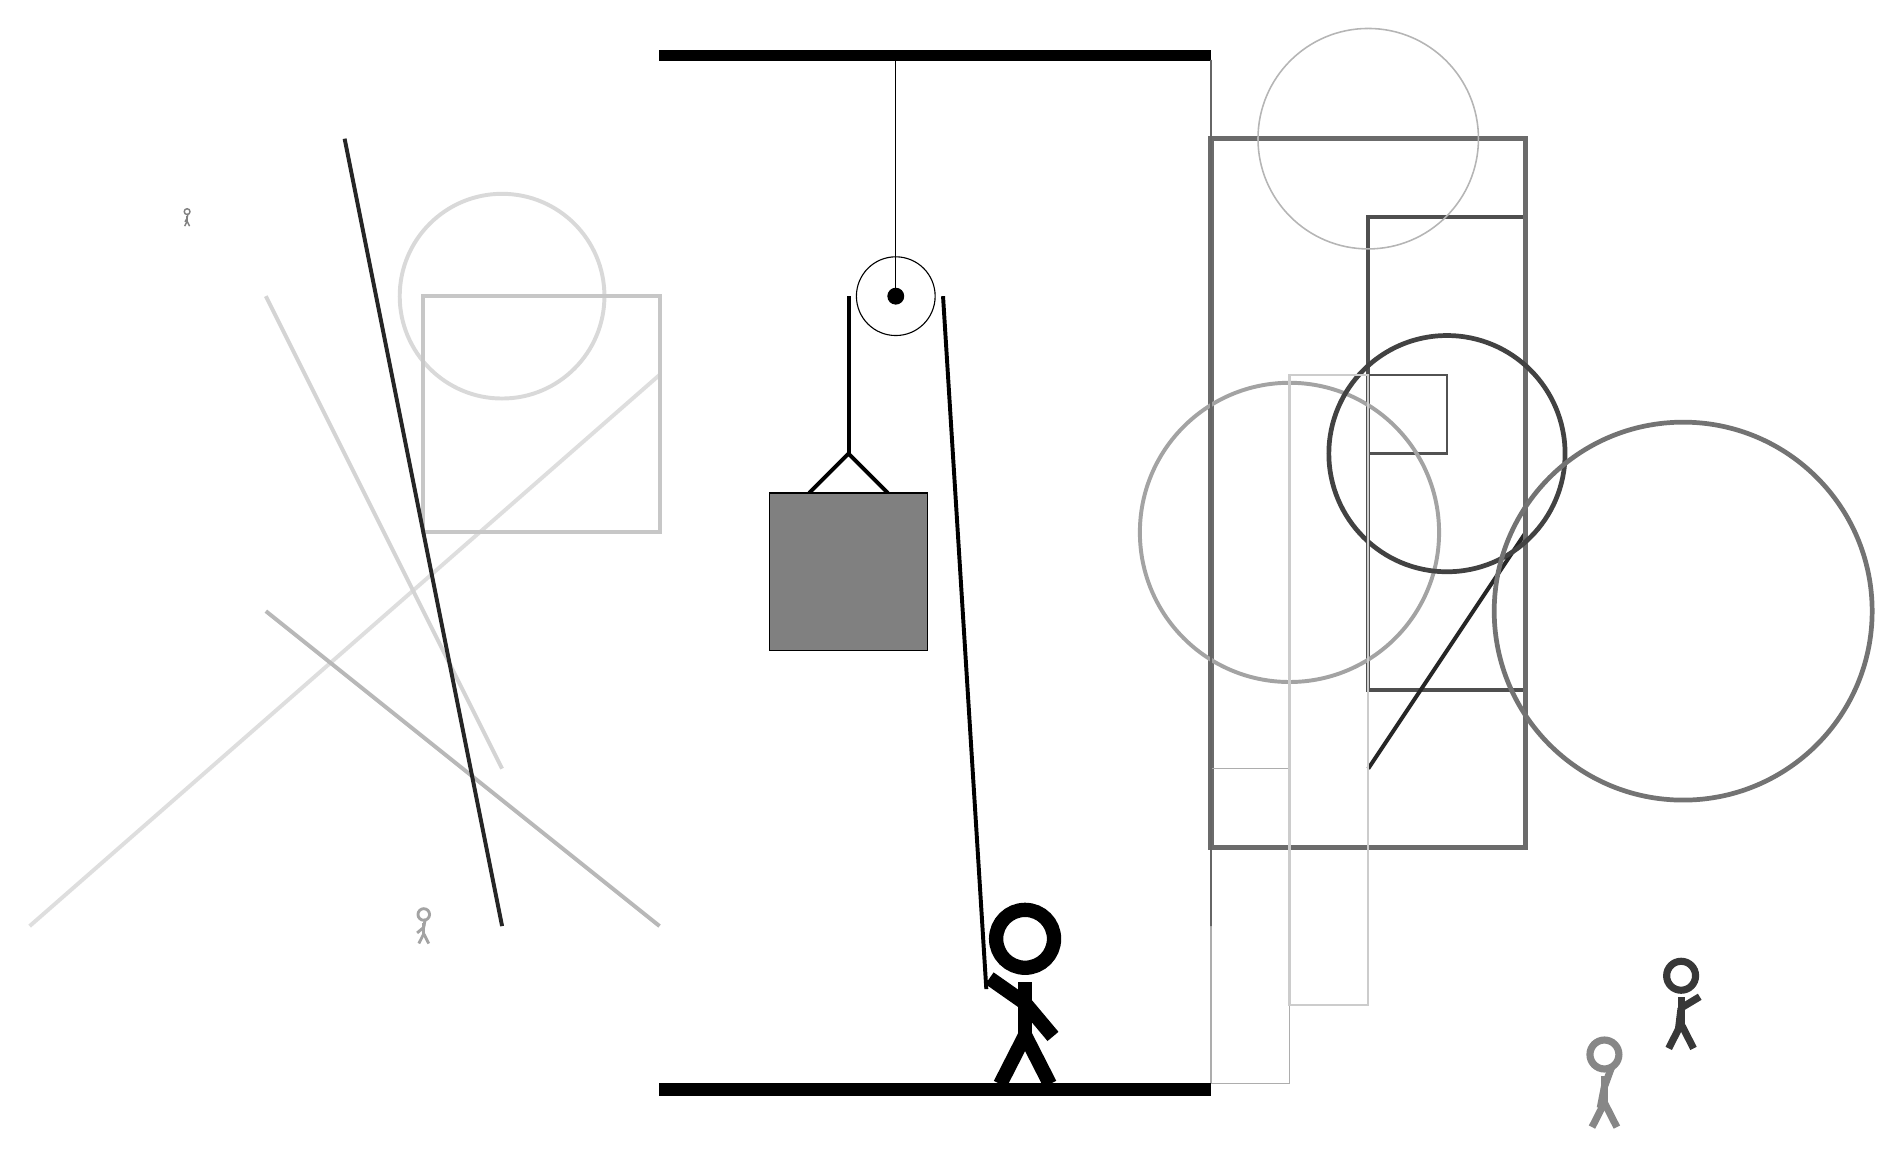
\begin{tikzpicture}
		%%%%% START %%%%%
		
		\draw[fill=black] (-2, 10) rectangle (5, 10.125);
		
		\draw (1, 7) circle (0.5);
		\draw[fill=black] (1, 7) circle (0.1);
		\draw (1, 10) -- (1, 7);
		
		\draw[line width=0.5mm] (-0.1, 4.5) -- (0.4, 5.0) -- (0.9, 4.5);
		\draw[fill=black!50] (-0.6, 4.5) rectangle (1.4, 2.5);
		
		\draw[line width=0.5mm, color=black!13](-2, 6) -- (-10, -1);
		
		\draw[line width=0.5mm, color=black!69] (7, 8) rectangle (9, 2);
		\node[line width=0.4mm, color=black!50] at (-8, 8) {\Strichmaxerl[1][61][79]};
		\draw[line width=0.3mm, color=black!68] (7, 5) rectangle (8, 6);
		\draw[line width=0.5mm, color=black!85](9, 4) -- (7, 1);
		\draw[line width=0.5mm, color=black!28](-7, 3) -- (-2, -1);
		\draw[line width=0.5mm, color=black!17](-7, 7) -- (-4, 1);
		\node[line width=0.7mm, color=black!36] at (-5, -1) {\Strichmaxerl[2][40][80]};
		\draw[line width=0.7mm, color=black!58] (5, 0) rectangle (9, 9);
		\draw[line width=0.2mm, color=black!32] (5, 1) rectangle (6, -3);
		\draw [line width=0.5mm, color=black!15](-4, 7) circle (1.3);
		\node[line width=0.7mm, color=black!47] at (10, -3) {\Strichmaxerl[5][79][70]};
		\draw [line width=0.5mm, color=black!36](6, 4) circle (1.9);
		\draw[line width=0.5mm, color=black!22] (-2, 4) rectangle (-5, 7);
		\draw[line width=0.5mm, color=black!85](-4, -1) -- (-6, 9);
		\node[line width=0.5mm, color=black!78] at (11, -2) {\Strichmaxerl[5][83][31]};
		
		\draw [line width=0.2mm, color=black!29](7, 9) circle (1.4);
		
		\draw[line width=0.3mm, color=black!60] (5, 10) rectangle (5, -1);
		\draw [line width=0.6mm, color=black!74](8, 5) circle (1.5);
		
		\draw [line width=0.6mm, color=black!55](11, 3) circle (2.4);
		\draw[line width=0.3mm, color=black!20] (6, -2) rectangle (7, 6);
		
		
		\draw[line width=0.5mm] (0.4, 7) -- (0.4, 5.0);
		\centerarc[line width=0.5mm](1, 7)(0:180:0.6);
		\draw[line width=0.5mm](1.6, 7) -- (2.15, -1.8);
		
		\node at (2.6, -1.9) {\Strichmaxerl[10][-35][-50]};
		
		\draw[fill=black] (-2, -3) rectangle (5, -3.15);
		
		%%%%% END %%%%%
	\end{tikzpicture}
\end{document}